\chapter{The Solution}

The purpose of this chapter is to clearly identify, discuss, and justify the decisions you make
Depending on your type of project, you may not need to include all of these:


\section{Architectural Level}


\begin{figure}[h]
    \centering
    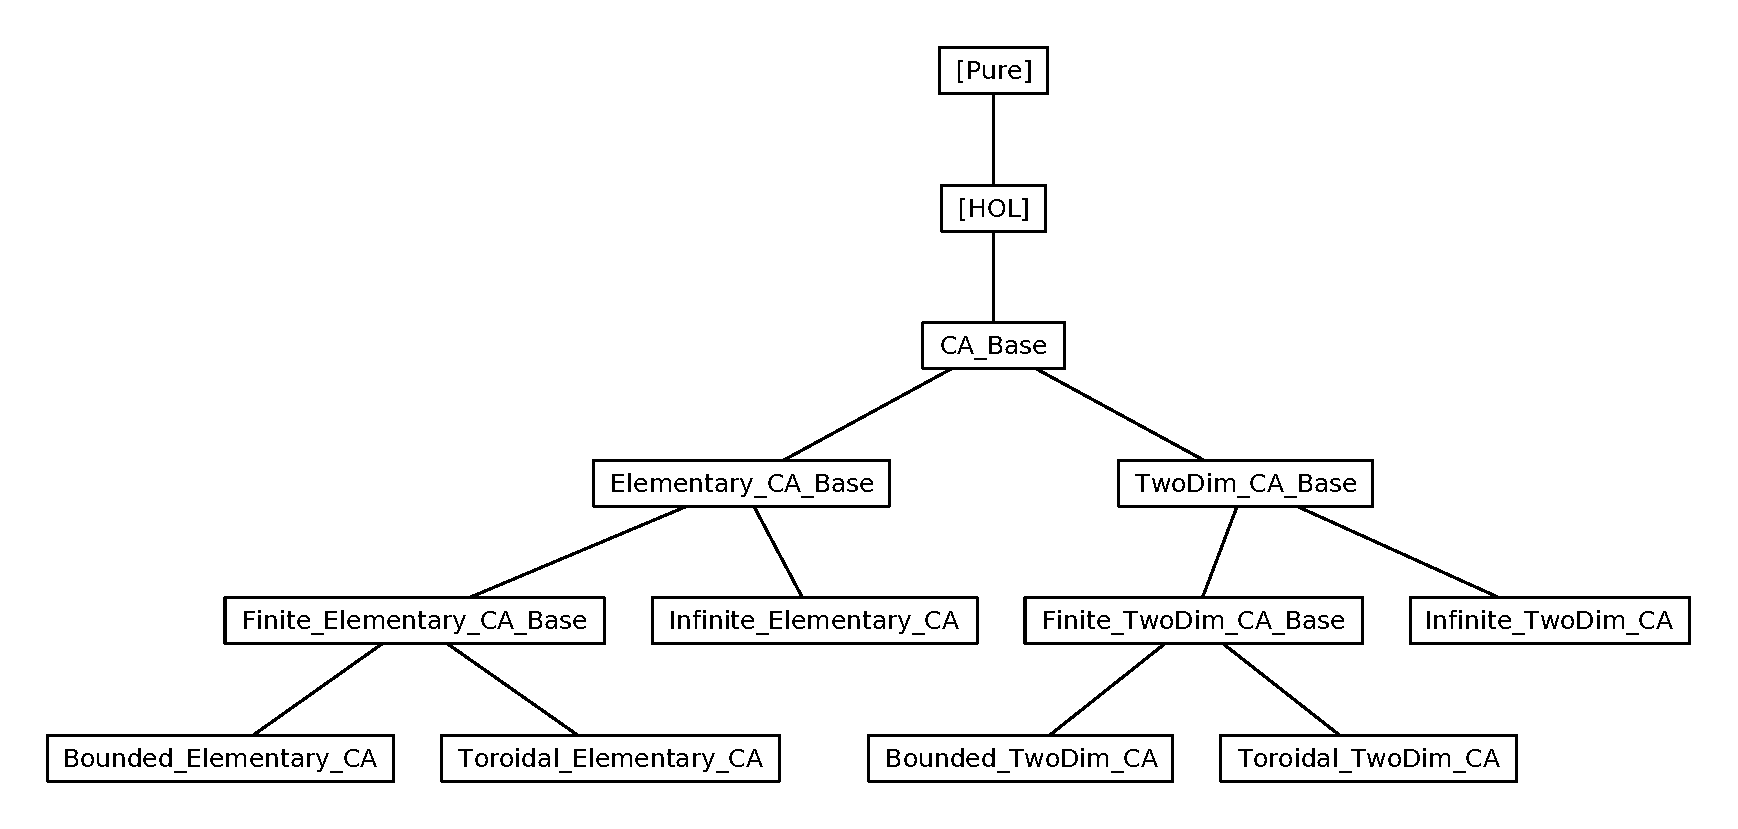
\includegraphics[scale=0.62]{session_graph.pdf}
    \caption{Dependency graph of project Theories}
    \label{fig:graph}
\end{figure}

\Cref{fig:graph} represents the overall architecture of dependencies of the various theory files in the project,
with files further down the tree depending on those above.
\mintinline{isabelle}{[Pure]} and \mintinline{isabelle}{[HOL]} contain the base definitions necessary to do work in Isabelle,
all the rest are new theories created for the project.

From the simplest core definitions given in \mintinline{isabelle}{CA_Base},
the project essentially splits into two due to the differences in implementing one dimensional versus two dimensional CA.
However the internal structure of these two subtrees are exactly the same apart from the distinction in dimension.
They both contain a base file for the two kinds of finite CA,
and another file dealing with the infinite case.

Each of the six root nodes contains the definition of one of the six distinct kinds of CA realised in the project.
They very roughly increase in power and complexity from left to right.

\section{Analytical Work}

E.g. Equations, etc. that describe your solution


\section{High Level}

E.g. Packages, Class Diagrams, etc.


\section{Low Level}

E.g. Method specifications, Algorithms, etc.


\section{Implementation}

Discuss anything interesting here; put full source code in an appendix or attachment
